% \documentclass[preview]{standalone} % for final output:
\documentclass[preview,border=1mm]{standalone} % Adjust border as needed
% \documentclass[landscape]{article}
% \usepackage[margin=0.1in]{geometry} % Adjusts the margins and sets landscape mode
\usepackage{graphicx} % Required for inserting images

\usepackage{amsmath,amssymb,amsthm}
\usepackage{tikz}
\usetikzlibrary{matrix}

\begin{document}


\begin{center}
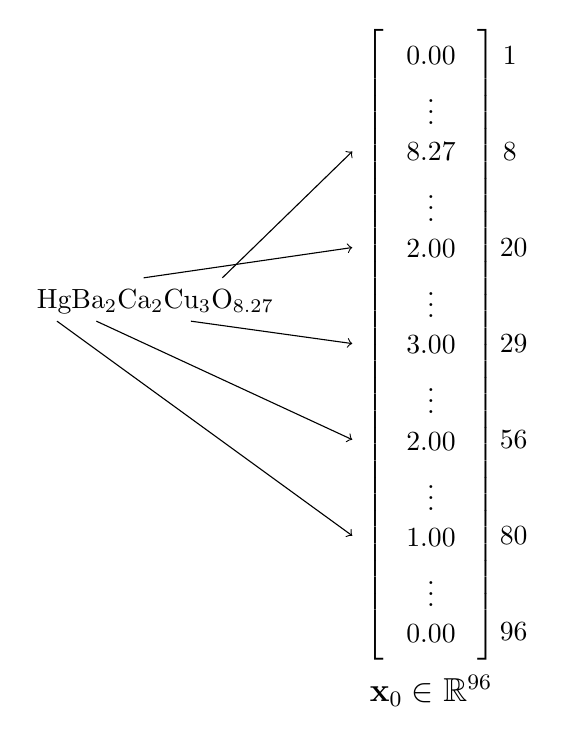
\begin{tikzpicture}
    \node at (0,-0.45) {$\mathrm{HgBa_{2}Ca_{2}Cu_{3}O_{8.27}}$};
    
    
    \draw[->] (0.85,-0.15) -- (2.5,1.455);
    \draw[->] (-0.15,-0.15) -- (2.5,0.235);
    \draw[->] (0.45,-0.7) -- (2.5,-0.985);
    \draw[->] (-0.75,-0.7) -- (2.5,-2.205);
    \draw[->] (-1.25,-0.7) -- (2.5,-3.425);
    

    %%%%%%%%%%%%%%%%%%%%%%%%%%%%%%%%%%%%
    % TikZ matrix replacing the big rectangle
    %%%%%%%%%%%%%%%%%%%%%%%%%%%%%%%%%%%%
    \matrix (m) at (3.5, -1) [matrix of nodes, left delimiter={[},right delimiter= {]}]
    {
        0.00 \\
        $\vdots$ \\
        8.27 \\
        $\vdots$ \\
        2.00 \\
        $\vdots$ \\
        3.00 \\
        $\vdots$ \\
        2.00 \\
        $\vdots$ \\
        1.00 \\
        $\vdots$ \\
        0.00 \\
    };

    \node at (4.5, 2.675) {1};
    \node at (4.5, 1.455) {8};
    \node at (4.55, 0.235) {20};
    \node at (4.55, -0.985) {29};
    \node at (4.55, -2.205) {56};
    \node at (4.55, -3.425) {80};
    \node at (4.55, -4.645) {96};

    \node at (3.5, -5.4){\large $\mathbf{x}_0 \in \mathbb{R}^{96}$};
    

\end{tikzpicture}
\end{center}



\end{document}
